%% -*- coding:utf-8 -*-
\begin{figure}
\centering
\ifpdf
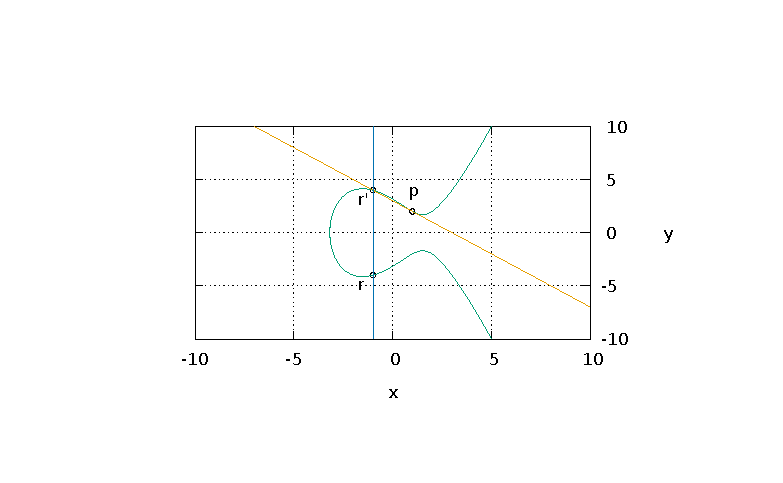
\includegraphics[angle=0,scale=1.5]
{./add/discretmath/picellipticsumeq2.pdf}
\else
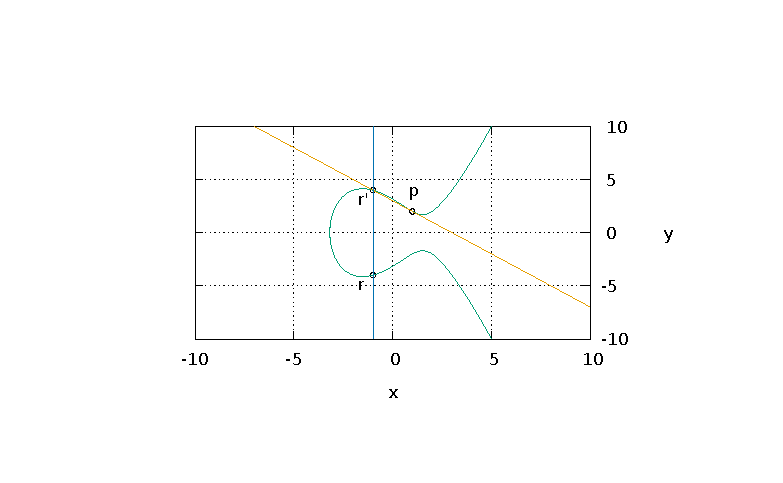
\includegraphics[angle=0,scale=1.5]
{./add/discretmath/picellipticsumeq2.eps}
\fi
\caption{Эллиптическая кривая $y^2 = x^3 -7 x + 10$ над полем
  вещественных чисел $\mathbb{R}$. Сложение двух точек с одинаковыми
  координатами $p(1,2)$: $2p = r (-1,-4)$}
\label{fig:add:ellipticRsumEq2}
\end{figure}
